\section{Steam Systems and Component Models}\label{steam-systems-and-component-models}

A steam system uses the vapor phase of water to supply enthalpy or kinetic energy through the piping network.~ In case of EnergyPlus, the steam system is designed to provide energy solely for the building heating requirements.~ Hot steam from the boiler or steam generator in buildings can be used to heat a conditioned space with suitable heat transfer equipment such as fan-coils units, unit-heaters, radiators and convectors or steam can also heat water through shell and tube heat exchangers, and hot water can be supplied to the terminal units to provide the zone heating requirements.

The advantages that steam system offer over hot water or other heating systems are:

\begin{enumerate}
\def\labelenumi{\arabic{enumi}.}
\item
  Steam flows through the system unaided by external energy source such as pumps; pressure difference moves steam across the system.
\item
  Steam, because of its low-density, can be used in high-rise buildings where water systems create excessive pressure.
\item
  Terminal units such as heating coils can be added or removed without making any changes to the system.
\item
  Steam components can be repaired or replaced by closing the steam supply without the difficulties associated with draining and refilling like in the water systems.
\item
  Steam is pressure-temperature dependent, therefore the system temperature can be controlled by varying either steam pressure or temperature.
\item
  Steam can be distributed through out the system without any change in temperature.
\end{enumerate}

In view of the advantages mentioned, the steam systems are suitable for applications where heat is required for process and comfort heating such as in industrial plants, hospitals, restaurants, dry cleaning plants laundries and commercial buildings.~ They are also suitable in places where the heating medium has to travel great distances such as in facilities with scattered building locations or where the building height would result in excessive pressure in a water system, or locations where the load changes occur intermittently.~ Thus steam system is an essential and necessary development step for EnergyPlus.

From EnergyPlus simulation point of view, the advantage associated with a steam system is that steam can be distributed through out the system without change in temperature.~ This means that the boiler outlet temperature can simply be set equal to the heating coil inlet temperature for a steam system.

Another simulation-based advantage associated with the steam system is Steam Quality, which does not change from boiler outlet to coil inlet.~ Actual building steam systems are equipped with condensate drains through out the system, these drains remove, almost immediately any condensate that is formed during steam transportation, thereby maintaining the steam quality at constant value of 1.0 through out the high-pressure steam side.

The HVAC steam system implementation includes simulation models for two phase steam equipment like steam boiler, steam to air heating coils, steam pipes and condensate pumps, which can be connected to the generic loop framework.

\subsection{Steam Loop Assumptions}\label{steam-loop-assumptions}

To replicate the working of an actual building steam system in a satisfactory manner with simulation, it was necessary to make certain assumptions.~ These assumptions help simplify the loop complexity and increase usability.~ The effects of the assumptions made are described in detail below.

The following figure describes the Temperature Entropy Ts diagram based on which the steam system operates in EnergyPlus.~ The steam side of the loop operates on constant saturation pressure of steam: PSteam, the waterside of the loop operates at atmospheric pressure Patm.

\begin{figure}[hbtp] % fig 129
\centering
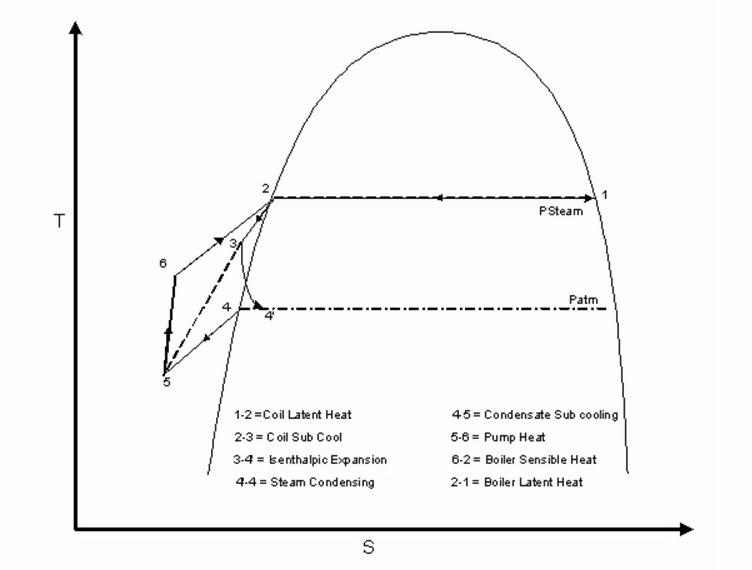
\includegraphics[width=0.9\textwidth, height=0.9\textheight, keepaspectratio=true]{media/image1986.png}
\caption{Schematic of Temperature – Entropy Diagram for Steam loop \protect \label{fig:schematic-of-temperature-entropy-diagram-for}}
\end{figure}

It should be noted that the figure is simply a schematic and not a scaled representation of the process on a Mollier Chart.~ For the following descriptions, please refer to the schematic figure above.

\begin{itemize}
\item
  ~Process 1--2 on the Ts diagram, represents condensation of steam in the coil at constant pressure; this is where the steam gives up latent heat to the zone.
\item
  ~Process 2--3 represents the subcooling of condensed steam at higher pressure, this subcooling takes place inside the steam coil, just before the steam trap.~ The delta temperature represented by 2-3 is the degree of subcooling in the steam coil, and is a user input to the steam coil.~ This subcool generally accounts for 1 to 2 \% of the total heat transfer in the steam coil.
\item
  ~Process 3--4' represents the isenthalpic expansion of water from high-pressure steam side to atmospheric pressure across the steam trap.~ As steam gives up its latent heat at the steam coil the condensate that forms in the steam coil still exists at higher pressure.~ This condensate is discharged to a lower pressure across the steam trap, this condensate contains more heat than necessary to maintain the liquid phase at the lower pressure, this excess heat causes some of the condensate to vaporize or flash to steam at lower pressure at some quality.~ The amount of water that flashes to steam can be calculated by the following equation
\end{itemize}

\begin{equation}
\% Flash\,\,Steam\,\, = \frac{{{h_{4'}} - \,{h_4}}}{{{h_{fg}}}}\,\, \times \,\,\,100
\end{equation}

Where h4' is Enthalpy of liquid at steam pressure just before condensate is supposed to leave the coil.~ Enthalpy at Point 3 is equal to enthalpy at point 4', since it is an isenthalpic process, and~ hfg is the latent enthalpy of the fluid at atmospheric pressure.

For example, water at 102LC and 120 Kpa flashes to steam at at100LC and atmospheric pressure, with quality equal to 0.003.~ This results in loss of some latent capacity of steam and is one of the terms contributing to loop loss in steam system.

\begin{itemize}
\item
  ~Process 4'- 4 represents the condensation of the flashed steam, which has exited from steam trap into the condensate drain.~ Condensation occurs at atmospheric pressure Patm, there is loss in latent capacity due to this unavoidable process, only condensate can be returned back to the boiler in a steam system.
\item
  ~Process 4-5 represents the loop sub cooling at atmospheric pressure; this is the sub cooling of the condensate that takes place during condensate return to the boiler because the return loop is not insulated, loop sub cooling is of the order of 20LC to 30LC.~ This is a user-defined input in every steam coil, because the variability in location of steam coils in a building will result in different condensate return temperatures for each of the coils.
\item
  ~Process 5-6 represents the temperature and pressure rise in condensate due to pump heat addition.~ The pumping process generates heat, which is added to the condensate.~ The condensate is pumped back to the boiler at higher pressure.
\item
  ~Process 6-2 represents the sensible heat addition by the boiler to the return condensate.
\item
  ~Process 2-1 represents the latent enthalpy of steam, added by the boiler to the water to convert it to steam at saturation pressure.
\item
  ~Point 3, which is outlet of the coil and Point 5, which is inlet of the pump are specified directly by the user, subsequently the loop losses in EnergyPlus are directly summed up as the enthalpy difference between point 3 and 5, which is calculated by fluid property routines in EnergyPlus.~ This helps to maintain flexibility and at the same time helps negate the intermediate points calculation in the system.
\end{itemize}

Aspects of the steam loop such as quality of steam, steam pressure, and steam generation which play an important role in EnergyPlus simulation are described in following sections.

\subsubsection{Constant Pressure Steam loop}\label{constant-pressure-steam-loop}

The steam loop in EnergyPlus is pressure driven and it is assumed to operate at constant pressure on the gaseous-steam part, while the condensate return loop is assumed to operate at atmospheric pressure.~ The steam loop essentially operates at saturation pressure corresponding to the steam temperature; the steam boiler serves to maintain the loop temperature.~ The boiler model determines the amount of energy required to generate the required amount of steam.

Factors such as friction in pipes, which tend to cause small amount of pressure drop in steam loop are neglected in the model.~ It is assumed that the steam pipes are fairly well insulated to prevent heat loss and subsequent condensation of steam in the pipes.~ In actual systems small quantities of steam, which condenses due to heat loss during transportation is removed immediately from the system by steam drains.~ This helps eliminate water hammer, degradation of steam quality and heat transfer capability.

\subsubsection{Steam Generation at Saturated Conditions:}\label{steam-generation-at-saturated-conditions}

Building steam heating systems avoid supplying superheated steam because superheat damages the building HVAC equipment.~ Superheated steam is generated only if there is a cogeneration power system in building such as steam turbine, which requires superheated steam.~ The purpose of having superheated steam is redundant for building steam heating systems because the amount of energy carried by the same is negligible compared to the latent heat. A simple enthalpy calculation, based on each unit of steam mass flow rate (1 kg/s), has been provided in this section to describe the negligible effect of superheat..

Case 1: Loop Operating at Saturation Conditions (no superheat), calculating enthalpy of saturated steam at boiler outlet temperature.

Boiler Outlet Temperature = 105BC,

\begin{equation}
{h_{Case1:NoSuperheat}} = [{h_f}_{{{105}^ \bullet }C}]
\end{equation}

\begin{equation}
{h_{Case1:NoSuperheat}} = \,\,\,\,2684000\,\,\,\,\,\,J
\end{equation}

Case 2: Loop operating with Superheated steam, calculating enthalpy of superheated steam for 5BC superheat.

Degree of Superheat = 5BC

Boiler Outlet Temperature = 110BC,

\begin{equation}
{h_{Case2:Superheat}} = [{h_f}_{{{110}^ \bullet }C}]
\end{equation}

\begin{equation}
{h_{Case2:Superheat}} = \,\,\,2691000\,\,\,\,\,\,\,\,J
\end{equation}

The energy difference between the superheated state and the saturated state as calculated in the following equation.~ A 5BC superheat provides only a 0.2608\% increase in heat transfer.~ The advantage of this additional increase in heat transfer is negligible, especially when considering the economic aspect of sizing a bigger heat exchanger to accommodate additional superheat transfer.~ The detrimental effects of superheated steam on the building HVAC system also come into effect once superheat is used.

\begin{equation}
\Delta {Q_{2 - 1}}\,\,\, = \,\,\,\frac{{2691000\, - 2684000}}{{2684000}}\,\, \times 100\,\,\,\, = \,\,0.2608\,\,\,percent
\end{equation}

Based on the reasoning above the steam loop in EnergyPlus is designed and implemented to operate at saturated conditions.

\subsubsection{Steam Quality}\label{steam-quality}

The boiler operation is assumed capable to generate steam at quality equal to1.0 every time.~ This is a reasonable assumption, since in practice the variability in generated steam quality would only occur if the boiler operation were not properly controlled.

The steam loop is assumed to have perfect transport mechanism.~ There is no transportation losses due to friction and heat transfer with surroundings.~ This assumption helps maintain the quality of steam through out the system constant value of either 0 or 1.

Steam enters the coils at boiler outlet conditions.~ Steam coils are designed with steam traps, which only allow condensed steam to leave the coil; hence the steam always condenses and leaves the coil at quality of 0.0.

With the above simplifying assumption enables the EnergyPlus steam loop to be solved without problems.

\subsubsection{Steam Traps}\label{steam-traps}

Steam traps are essential part of the steam system; they are indirect flow controllers of the loop.~ Purpose of steam trap is to allow only condensate out of the coil from higher-pressure steam to lower atmospheric pressure condensate return line.~ Points 3-4C, in schematic~ Figure~\ref{fig:schematic-of-temperature-entropy-diagram-for}, represent this process across the steam trap on the Ts diagram.~ The expansion process across the steam trap is assumed to be isenthalpic.~ There is possibility of flashing of high-pressure condensate across the trap because of pressure drop, resulting in generation of steam at lower pressure, this steam generated at lower pressure subsequently condenses in the return piping, and heat is lost to the atmosphere.~ This heat lost is a part of the steam loop losses.

Steam traps are modeled in the EnergyPlus steam coil by assigning the condensate outlet from the coil a quality of 0.0 and sub cooling the condensate at lower pressure.

Although condensate from the steam coil contains valuable heat, attempting to utilize this heat by holding the condensate in the coil reduces the heat transfer area.~ It causes operational problems because it retains air, which further reduces heat transfer and non-condensable gases such as carbon dioxide, which cause slow corrosion of the steam coil.~ Steam moves rapidly in mains and supply piping so when condensate accumulates to the point where the steam can push a slug of it, serious damage can occur from the resulting water hammer, hence the condensate should be immediately removed from the steam coil.~ This is achieved with steam traps.

Hence an ideal steam trap should remove all condensate, air, and non-condensable gases that might be in the system, with little or no loss of steam.

\subsubsection{Loop Losses}\label{loop-losses}

Subcooling of condensate in condensate return piping and flash steam condensing across the steam trap constitute the unavoidable loop losses in the EnergyPlus simulation steam system.~ These losses can be inferred from Figure~\ref{fig:schematic-of-temperature-entropy-diagram-for} and are summed up by calculating enthalpy difference between points 3 and 5 on the schematic Ts diagram.

Unavoidable losses in the EnergyPlus steam loop occur due to pressure drop across the steam trap, which causes flashing of steam and loss in some percentage of latent heat of steam, process 3-4' and 4'-4 on the Ts diagram in Figure~\ref{fig:schematic-of-temperature-entropy-diagram-for}.~ The condensate is pumped backed to the boiler through return pipe network, which is not insulated.~ Sub cooling of the condensate occurs in the return network, represented by process 4-5 on the Ts diagram in Figure~\ref{fig:schematic-of-temperature-entropy-diagram-for}.~ This loop sub cool contributes to significant percentage of loop losses.

In practical systems the return pipeline to the boiler is not insulated despite the condensate containing some valuable heat, however due to low mass flow rate of steam, this amount is negligible and only recovered if separate heat recovery systems are used by coupling them to the loop.~ The condensate is occasionally collected in a receiver and then pumped back to the boiler.~ EnergyPlus simulation mimics practical systems by assumed that the return pipeline is not insulated and accounts for this by calculating loop losses.

The loop losses are calculated in the steam coil simulation model rather that the steam pipe simulation, because the condensate sub cool in the return loop is a direct function of the location of the steam coil in the building.~ In building energy software like EnergyPlus the user would have a fair idea about location of steam coils rather than the location of condensate return piping.

\subsection{Steam To Air Heat Exchanger}\label{steam-to-air-heat-exchanger}

\subsubsection{Description of Model:}\label{description-of-model-001}

The steam to air heat exchanger (Coil:Heating:Steam input object) is the terminal equipment in the steam loop on the demand side that satisfies the heating requirements of the various zones.~ The steam-to-air heat exchanger simulation model in EnergyPlus calculates the mass flow rate of steam desired to meet the heating demand.

A heating coil can be used either as a zone coil or a coil in the air loop depending on the user and application.~ The steam coil simulation model is designed to take these two locations into consideration.~ An air-loop steam heating coil is temperature controlled and the zone coil is zone load controlled.~ This relatively simple and straightforward concept of coil control is preferred over the iterative method to determine mass flow rates using various numeric techniques.~ The assumptions made in the coil model are described in the section below.

This model accounts for the latent heat transfer and sensible cooling of water; the question of superheat is eliminated because steam is assumed to be saturation conditions.~ Steam enters the coil at quality equal to 1.0, at saturation temperature and leaves the coil with desired degree of sub cooling.~ The user inputs the desired degree of subcooling, which determines the condensate outlet condition from the coil.

EnergyPlus heat balance methods determine the amount of heating required in the zone to maintain the zone at the desired conditions.~ Based on this value of heating load, the zone coil determines the mass flow rate of steam required since the heating coil load is the control variable in a zone coil.~ The following equation describes this calculation to determine steam mass flow rate required for the desired heating capacity. The steam latent heat of vaporization, \emph{h}\(_{fg}\) and the condensate heat capacity, \emph{C}\(_{p,w}\) are evaluated at the steam coil inlet node temperature and standard barometric pressure of 101325.0 Pa.

\begin{equation}
{\dot m_{zc}}\,\,\,\, = \,\,\,\,\,\frac{{{Q_{zc}}}}{{{h_{fg}} + {c_{p,w}} \times \Delta {T_{sc}}}}
\end{equation}

In case of the air loop-heating coil, the load on the coil is calculated within the coil simulation routine.~ The air loop coil is setpoint controlled and heats the air to maintain the air stream at the desired setpoint, the setpoint is a user input, generally in the range of 12B C to 16BC. The following equation describes the air loop coil load.

\begin{equation}
{Q_{al}}\,\, = \,\,{\dot m_a}\,\,\, \times \,\,\,\,\,{c_{p,a}}\,\,\, \times \,\,\,\,\,\left[ {{T_{sp}}\,\,\, - \,\,\,{T_a}} \right]
\end{equation}

The following equation is used to determine the steam mass flow rate required by the air loop coil to meet the heating requirements.

\begin{equation}
{\dot m_{al}}\,\,\,\, = \,\,\,\,\,\frac{{{Q_{al}}}}{{{h_{fg}} + {c_{p,w}} \times \Delta {T_{sc}}}}
\end{equation}

Each of the zone coils and air loop coils are simulated independently and the steam mass flow rates for each is added over every time step of simulation.~ This value of total mass flow rate is reported to the boiler, which in turns supplies this required amount of steam.

The control of the steam to air coil is a complex issue.~ The loop splitter-splits total steam flow from the boiler and delivers the required amount of steam to each of the coils connected to the loop through the steam pipe network.~ In cases where the system is undersized, the coils demand more mass flow rate of steam than the boiler can generate.~ The splitter in this case cannot provide all the coils with requested steam mass flow.~ Subsequently the coils are starved of steam and the zone temperatures fall.~ In some cases the user might schedule off the coil, they should then not operate.~ These issues need to be taken care of in the implementation of the steam coil simulation model.~ The control algorithm for the steam coil operation under various situations is best explained with the help of pseudo-code using standard IF THEN ELSE blocks.

*********************PSEUDO CODE SECTION STARTS**************************

\subsubsection{Steam coil is zone load controlled.}\label{steam-coil-is-zone-load-controlled.}

\begin{equation}
IF\,\,\,\,\,(Coil\, = LoadControlled)\,\,\,\,\,\,THEN\,
\end{equation}

Check for operational conditions only then continue simulation further.~ The operational conditions are the inlet mass flow rates of steam and air to the coil, the user schedule to the coil and heating load on the coil.~ The coil is simulated only if these conditions are met.

\begin{equation}
IF\,\,\,\left[ {\,({{\dot m}_s}\,\,\, > \,\,\,0)\,\,.\,\,\,and.\,\,\,({{\dot m}_a} > \,\,\,0)\,\,.and.\,\,(Schedule\,\, = \,\,\,ON)\,.and.\,\,\,({Q_{ZC}}\,\, > \,\,0.0)\,} \right]\,\,\,THEN
\end{equation}

If the heating demand from the zone-heating coil is greater than coil capacity, then the heating coil is undersized, and the coil can only deliver its maximum heating capacity to the zone.~ In this case the heating demand on the coil is set equal to this lower value of maximum heating capacity.~ If the above is not true then the simulation ignores this statement and proceeds to the next one.

\begin{equation}
IF\,\,\,\left[ {\,\,\,({Q_{ZC}}\,\, > \,\,{Q_{Z{C_{Max}}}})} \right]\,\,\,\,\,\,THEN\,\,\,\,\,\,\left[ {{Q_{ZC}} = \,\,{Q_{Z{C_{Max}}}}} \right]
\end{equation}

The following equation calculates the steam mass flow rate required by the coil.~ This flow rate is required to meet the heating requirements for the zone.~ This value of mass flow is requested from the splitter outlet.

\begin{equation}
{\dot m_{zc}}\,\,\,\, = \,\,\,\,\,\frac{{{Q_{zc}}}}{{{h_{fg}} + {c_{p,w}} \times \Delta {T_{sc}}}}
\end{equation}

If the calculated value of steam mass flow with the previous equation is greater than the maximum inlet steam flow that the splitter can provide to the coil at that time step.~ Then the requested coil flow rate is set equal to the inlet steam flow rate.~ This is the maximum amount of steam that can be supplied to the coil at this moment.~ The coil can provide heating capacity equal to this limited amount of steam.~ If the requested flow rate is less that what the splitter can provide then the program ignores the logic of the IF Loop Below

\begin{equation}
IF\,\,({\dot m_{zc}}\,\, > \,\,{\dot m_{in}})\,\,THEN\,\,(\,\,\,{\dot m_{zc}}\,\, = \,\,{\dot m_{in}})
\end{equation}

Re-Calculating the coil heating capacity with the lower value of steam mass flow rate.

\begin{equation}
{Q_{ZC}} = {\dot m_{zc}}\,\, \times \,\,({h_{fg}} + {c_{p,w}} \times \Delta {T_{sc}})
\end{equation}

\begin{equation}
END\,\,IF
\end{equation}

The following equations calculate the outlet condensate-water and outlet air temperatures to the zone based on the amount of heating capacity provided by the coil.

\begin{equation}
T{w_{out}} = \,\,T{s_{in}}\,\, - \,\,\,\Delta {T_{sc}}
\end{equation}

\begin{equation}
T{a_{out}}\,\,\, = \,\,T{a_{in}}\,\, + \,\,\,\frac{{{Q_{zc}}}}{{\,{{\dot m}_a}\, \times \,\,\,{c_{p,a}}}}
\end{equation}

\(ELSE\) Else the coil is not running and in this case set outlets to inlets.

\begin{equation}
{\dot m_s} = 0\,,\,\,\,{\dot m_a} = 0\,,\,\,\,\,\,\,\,\,\,\,\,\,{Q_{zc}} = 0,\,\,\,\,\,\,\,\,\,\,\,\,T{w_{out}} = T{s_{in\,\,,\,\,\,\,}}\,\,\,\,\,\,T{a_{out}} = T{a_{in}}
\end{equation}

\begin{equation}
END\,\,IF
\end{equation}

\(END\,\,IF\) ~End IF for the zone load controlled coil.

\subsubsection{Steam coil is temperature controlled.}\label{steam-coil-is-temperature-controlled.}

\begin{equation}
IF\,\,\,\,\,(Coil\, = TemperatureControlled)\,\,\,\,\,\,THEN\,
\end{equation}

Check for operational conditions and continue simulation further.~ The operational conditions are the inlet mass flow rates of steam and air to the coil, the user schedule to the coil and delta temp exists between the setpoint and air inlet temperature.~ The coil is simulated only if these conditions are met.

\begin{equation}
IF\,\left[ \begin{array}{l}\,({{\dot m}_s}\,\,\, > \,\,\,0)\,\,.\,and.\,({{\dot m}_a} > \,\,\,0)\,\,.and.\,\,(Schedule\,\, = \,\,\,ON)\,.and.\,\\\,\,({T_{SP}} - T{a_{in}})\,\, > \,\,0.0001)\,\end{array} \right]\,THEN
\end{equation}

Calculate the heating load on the coil using setpoint and inlet air temperatures.

\begin{equation}
{Q_{al}}\,\, = \,\,\,{\dot m_a}\, \times \,\,\,C{p_a}\,\, \times \,\,\,\,[\,\,{T_{sp}}\,\, - \,\,\,{T_a}]
\end{equation}

The logic loop for temperature-controlled coil begins here.~ In case the heating load on the coil is negative, which might occur if the setpoint is below the air inlet temperature, the coil operation needs to be shut off.

\begin{equation}
IF\,\,({Q_{al}}\,\,\, < \,\,\,\,0.0)\,\,\,\,THEN
\end{equation}

Assigning the inlet to outlet and mass flows to zero shuts off the coil operation.

\begin{equation}
{\dot m_s} = 0\,,\,\,\,{\dot m_a} = 0\,,\,\,\,\,\,\,\,\,\,\,\,\,{Q_{al}} = 0,\,\,\,\,\,\,\,\,\,\,\,\,T{w_{out}} = T{s_{in\,\,,\,\,\,\,}}\,\,\,\,\,\,T{a_{out}} = T{a_{in}}
\end{equation}

If air loop coil load is greater than maximum coil load calculated at maximum steam mass flow rate, in such case the coil is undersized, the coil can only deliver to the air loop its maximum heating capacity.~ Setting the air loop coil load equal to maximum load on coil.~ If this is not the case then the program ignores this ELSE IF block and proceeds to the next one.

\begin{equation}
ELSE\,\,\,IF\,\,\,\,\left[ {\,\,\,({Q_{al}}\,\, > \,\,{Q_{a{l_{Max}}}})} \right]\,\,\,\,\,\,THEN\,\,\,\,\,\,\left[ {{Q_{al}} = \,\,{Q_{a{l_{Max}}}}} \right]
\end{equation}

If the heating coil is under sized then it can only provide its maximum heating capacity, in this case the air temperature will be below the setpoint, and is calculated based on this maximum allowed value of heat transfer.~ Calculating the air and water outlet temperatures.

\begin{equation}
T{a_{out}}\,\,\, = \,\,T{a_{in}}\,\, + \,\,\,\frac{{{Q_{al}}}}{{\,\,{{\dot m}_a}\, \times \,\,\,{c_{p,a}}}}
\end{equation}

\begin{equation}
T{w_{out}} = \,\,T{s_{in}}\,\, - \,\,\,\Delta {T_{sc}}
\end{equation}

Determining the mass flow rate of steam required by the undersized coil.~ This value of mass flow is requested from the splitter outlet.

\begin{equation}
{\dot m_{al}}\,\,\,\, = \,\,\,\,\,\frac{{{Q_{al}}}}{{{h_{fg}} + {c_{p,w}} \times \Delta {T_{sc}}}}
\end{equation}

A check is introduced to determine if this requested mass flow rate is greater than what the splitter outlet can provide to the coil at that particular time step of simulation.~ In this case the requested value of steam mass flow is greater that what the splitter can provide to that coil, subsequently set the requested coil flow rate equal to the inlet steam flow rate, delivered to the coil by the splitter.~ This is the maximum amount of steam that can be supplied to the coil at this moment.~ If the requested flow rate is less that what the splitter can provide then the program ignores the logic of the IF Loop.

\begin{equation}
IF\,\,\,({\dot m_{al}}\,\, > \,\,{\dot m_{in}})\,\,THEN\,\,(\,\,\,{\dot m_{al}}\,\, = \,\,{\dot m_{in}})
\end{equation}

Re-Calculating the coil heating capacity and air outlet temperature with the lower value of steam mass flow rate provided by the splitter.

\begin{equation}
{Q_{al}}\,\,\,\, = \,\,\,\,{\dot m_{al}}({h_{fg}} + {c_{p,w}} \times \Delta {T_{sc}})
\end{equation}

\begin{equation}
T{a_{out}}\,\,\, = \,\,T{a_{in}}\,\, + \,\,\,\frac{{{Q_{al}}}}{{\,\,{{\dot m}_a}\, \times \,\,\,{c_{p,a}}}}
\end{equation}

\begin{equation}
End\,\,\,IF
\end{equation}

If the above two IF ELSE block are not true, then the coil is perfectly sized, the splitter can provide the required mass flow rate to the coil, and the setpoint temperature can be maintained as desired.

\begin{equation}
ELSE
\end{equation}

The ideal case where the coils can meet the required setpoint temperature.~ Setting the outlet air temperature to the setpoint, calculating the water outlet temperature and the required steam mass flow rate.

\begin{equation}
T{a_{out}}\,\,\, = \,\,{T_{SP}}
\end{equation}

\begin{equation}
T{w_{out}} = \,\,T{s_{in}}\,\, - \,\,\,\Delta {T_{sc}}
\end{equation}

\begin{equation}
{Q_{al}}\,\, = \,\,\,{\dot m_a}\, \times \,\,\,{c_{p,a}}\,\, \times \,\,\,\,[\,\,{T_{sp}}\,\, - \,\,\,{T_a}]
\end{equation}

\(END\,\,IF\) ~~ End IF statement, for the air coil heating loop.

\(END\,\,IF\) ~~~~~~~~ End IF statement for the operating condition loop

\(END\,\,IF\) ~~ End IF statement for the Temperature Setpoint Controlled Coil

The steam coil model encapsulates the above described control logic along with the other necessary simulation code for reading the user inputs and the code for reporting the simulation results.

*********************PSEUDO CODE SECTION ENDS**************************

The two main types of coil control discussed above are followed by common simulation code in the coil model.~ This code calculates the loop losses occurring due to flashing of steam across the steam trap, isenthalpic expansion occurring across the steam trap due to pressure difference, and loss occurring due to condensate sub cooling returning back to the boiler.~ The above-mentioned two processes are explained in Figure~\ref{fig:schematic-of-temperature-entropy-diagram-for} as process 3-4' and 4-5.

The loop loss calculation is included in the steam coil simulation model, because the degree of subcooling in the return piping for the condensate is solely a function of the coil location.~ In practical applications a coil, which is further away from boiler would return back condensate at much lower temperatures compared to coil, which is closer to boiler.~ Hence for user ease it makes perfect sense to include this input into the coil and calculate the pump inlet conditions in the steam coil simulation model itself.

The loop losses in the EnergyPlus steam system is calculated by determining the enthalpy difference between point 3 and 5.~ The simulation code that determines the loop loss is common to both the coil models, this helps determine the condensate pump inlet conditions.

The following equation is used to calculate condensate enthalpy at coil outlet, point 3 in Figure~\ref{fig:schematic-of-temperature-entropy-diagram-for}.~ Point 2 represents condensed steam; enthalpy at this point is calculated directly by EnergyPlus property routines.

\begin{equation}
{h_{f3}} = {h_{f2}} - {c_{p,w}} \times \Delta {T_{SC}}
\end{equation}

Point 4 is at atmospheric pressure, enthalpy at this is calculated directly by EnergyPlus property routines.~ It is saturation enthalpy of steam at quality equal to 0.0 and saturation temperature at atmospheric pressure.

Point 5 is inlet to the pump; enthalpy at this point is calculated with the following equation~ The delta temperature represents the degree of loop subcooling occurring during condensate return back to the pump.

\begin{equation}
{h_{f5}} = {h_{f4}} - {c_{p,w}} \times \Delta {T_{LSC}}
\end{equation}

Subsequently loop loss for each coil would be enthalpy difference between 3 and 5 and is calculated using the following equation

\begin{equation}
\Delta {Q_{loss}} = {\dot m_s}\,\,\, \times \,\,\,\,({h_{f3}} - {h_{f5}})
\end{equation}

The total loop loss would be a summation of the individual losses occurring for each of the steam coils, this is the unavoidable loss in current steam system.

A simple schematic describing the coil framework, inlet and outlet conditions to the coil and the flow rate resolution is shown in Figure~\ref{fig:schematic-of-steam-coil-connection-to}.~ Five zone coils and one air loop coil are described in the picture, Qzone is calculated by EnergyPlus heat balance and it is the input to the zone coils, while in air loop coil the Qal is calculated within the simulation model

\begin{figure}[hbtp] % fig 130
\centering
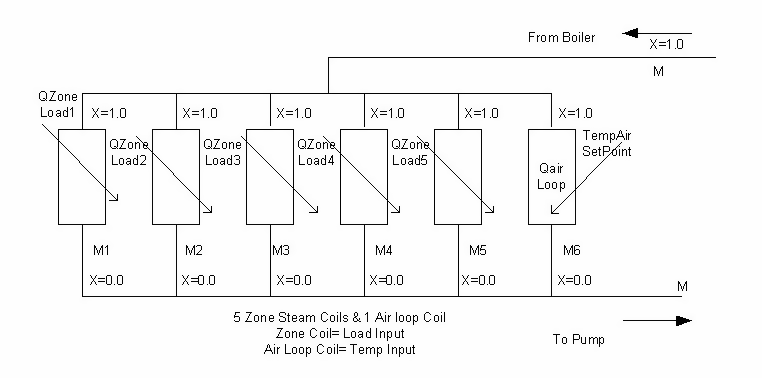
\includegraphics[width=0.9\textwidth, height=0.9\textheight, keepaspectratio=true]{media/image2032.png}
\caption{Schematic of Steam Coil Connection to the Steam Loop \protect \label{fig:schematic-of-steam-coil-connection-to}}
\end{figure}

As depicted in the figure above the steam condenses on entering the coils, sub cools by the specified amount and leaves the heat exchanger as water.~ The steam in the heat exchanger at any moment has to condense eventually since steam trap at the outlet to coil permits only water to leave the coil.~ Steam traps being an essential part of the loop are modeled by controlling the coil outlet condition at quality equal to 0.0.~ Subsequently the amount of heat transferred to air is a direct function of latent heat and the degree of sub cooling desired by the user.

\subsubsection{Model Assumptions}\label{model-assumptions-001}

The steam coils works on two basic assumptions, firstly, it's assumed that perfect latent heat transfer takes place over every time step, secondly, the user specified degree of subcooling occurs in the coil.~ Steam coils always use steam traps- purpose of which is to only let water out of the coil, hence the modeler knows with certainty the outlet dryness faction of steam coil is at quality equal to 0.0, because water leaves coil.~ Hence the heat transfer is equal to latent heat of steam, which is independent of UA value of coil when averaged over time step of EnergyPlus simulation.

In practice there is 1\% to 2 \% sub cooling of the outlet water stream, the user with desired degree of subcool input accounts for this, subsequently UA calculation for the coil model become superfluous and is neglected in the EnergyPlus model.

Ideally for sub-cooling UA would play an important role, however sub cooling in steam coil constitutes negligible amount of heat transfer, hence this model avoids the UA calculation.~ This is a very reasonable assumption since sensible heat transfer is barely 1\% to 2 \% of the total heat transfer in steam coils, simply due to large latent heat capacity of coil. NOTE in his thesis he gives a little example here which is probably not necessary for the Docs.

\subsection{Condensate Pump}\label{condensate-pump}

The steam loop operates at a pressure differential over the gaseous and liquid part of the loop; subsequently a condensate pump is required to pump the condensed steam back to the boiler at the required pressure.~ Two main reasons for condensed steam to be returned to the boiler is energy savings in reheating water since the water is at high temperature, secondly the water is treated by chemicals to prevent corrosion in the pipes and equipment.~ This is an expensive process and therefore it's economical to reuse the chemically treated water.

\subsubsection{Description of Pump Model}\label{description-of-pump-model}

The pump model designed in EnergyPlus is a variable speed condensate pump.~ Condensation of steam produces water, this takes place at variable rate hence the return water flow rate would be variable but constant when averaged over a time step.~ Condensate pumps operate intermittently; the pump will run at its capacity if a load/flow rate is sensed and will shut off if there is no load on the loop.

The condensate pump essentially operates between maximum and minimum flow rates, which are the physical limits of the device.~ The pump is designed to meet the flow request made by demand side components, which are the coils in case of steam system.

The main difference between the variable volume pump and the constant volume pump is the Part Load Performance Curve.~ The fraction of full load power is determined by the third order equation, which follows:

\begin{equation}
{P_{Frac}}\,\, = \,\,{C_1} + \,{C_2} \times PLR\,\, + \,\,\,{C_3} \times PL{R^2}\,\, + \,\,{C_4} \times PL{R^3}
\end{equation}

In preceding equation, PLR stands for part load ratio while C1 to C4 are pump- part load coefficients.~ The following five equations describe the pump operation and calculation of pump output variables such as total power, shaft power and pump heat to fluid etc.

\begin{equation}
\dot V\,\, = \,\,\frac{{\,\dot m\,}}{{{\rho_w}}}
\end{equation}

Using the previous equation the pump volume flow rate is determined; the user enters the value of the maximum and minimum volume flow rate.

The pump part load ratio is a function of the pump volume flow rate at any instance determined by the loop and the pump nominal volume flow rate, which is a user input.~ The following equation calculates the Part Load Ratio (PLR).

\begin{equation}
PLR = \,\frac{{\dot V}}{{{{\dot V}_{nom}}}}
\end{equation}

The pump power is calculated as described in following equation.~ Pump power is a product of fractional full load power and pump nominal power use.~ Fractional full load power is calculated in a preceding equation while pump nominal power is a user input to the model.

\begin{equation}
P = {P_{Frac}} \times {P_{Nom}}
\end{equation}

The shaft power is simply the product of the pump power and motor efficiency, this is required to calculate the heat generated and delivered to the fluid being pumped.~ The following equation is used to calculate pump shaft power.

\begin{equation}
{P_S}\,\,\, = P\,\,\,\, \times \,\,\,\,{\eta_m}
\end{equation}

The model assumes that all heat generated and lost ends up in the fluid to the loop, this assumption is necessary since EnergyPlus operates on a closed loop.~ The following equation is used to calculate the pump heat to the fluid, which raises the condensate temperature.~ The pump motor efficiency is defined by the user input and the fractional motor loss to fluid is the amount of heat generated by the pump motor that is added to the fluid loop (as opposed to being lost to the environment where the pump is located).~ FracMotorLossToFluid is also a user input

\begin{equation}
{P_H} = {P_S}\,\,\, + \,(\,P\,\, - {P_S}) \times {F_{mf}}
\end{equation}

The shaft power relates to the increase in head through the pump to the loop operating pressure.~ The head lost through the piping network due to frictional heat, represents the heat gain by the fluid throughout the network.~ .~ For model simplicity, this heat is added along with the heat resulting from the pump motor.~ The difference between the pump power and the shaft power is the inefficiency of the pump, or the amount of energy input into the pump that the motor converts to heat rather than mechanical energy.~ Some of this heat is added to the fluid being pumped.~ These two above-mentioned terms are used in the PumpHeatToFluid equation for calculating P\(_{H}\) shown above.

A simple energy balance over the pump based on the pump inlet conditions and flow rate is used to calculate the pump outlet temperature.~ The condensate outlet temperature from the pump is slightly higher than inlet due to the heat dissipation to the fluid steam during pumping action.~ This is calculated in the following equation.~ The pump water outlet temperature is the boiler inlet temperature.

\begin{equation}
{T_{{w_{out}}}} = {T_{{w_{in}}}}\,\,\, + \,\,\,\,\,\frac{{{P_H}}}{{\,\dot m\,\,\, \times \,\,\,\,{c_{p,w}}}}
\end{equation}

Pump control is an important part of the steam loop.~ Existing control structure from EnergyPlus has been utilized to operate the condensate pump.~ The pump is simulated first on the supply side of the loop after the demand side loop has determined what the demand on the loop will be.

A simple schematic describing the flow across the pump is shown in the following figure

\begin{figure}[hbtp] % fig 131
\centering
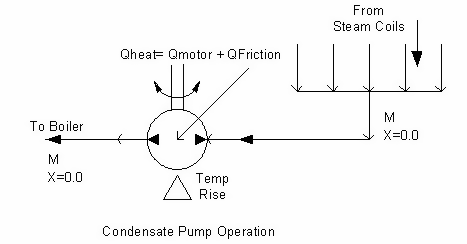
\includegraphics[width=0.9\textwidth, height=0.9\textheight, keepaspectratio=true]{media/image2040.png}
\caption{Schematic of Condensate Pump in Steam Loop \protect \label{fig:schematic-of-condensate-pump-in-steam-loop}}
\end{figure}

\subsubsection{Model Assumptions}\label{model-assumptions-1}

Due to the fact that a pump is a mechanical device that acts on the fluid it is circulating, it causes the fluid temperature rise.~ The EnergyPlus model assumes that all pressure increase caused by the pump will eventually be lost due to friction, and that friction will be added as heat to the fluid.~ Although the plant and condenser loops in steam systems are simple pressure-based models, a simplifying assumption has be made in EnergyPlus to assume the heat resulting from the pump itself and from friction throughout the loop is added at the fluid being pumped.~ In case of steam, this assumption is easily justified because the volume flow rate of water is very small in the loop.

\subsection{Steam Pipe}\label{steam-pipe}

\subsubsection{Description of Model}\label{description-of-model-1}

The steam pipe essentially serves as ``energy carrier'' and transfers the node conditions from one point of the pipe to another.~ It's simply a node inlet to node outlet connection, transferring values from inlet to outlet.~ The pipe forms an important part of the framework connecting various equipments from the supply to demand side and inlet and outlets of the equipments.

The steam pipe supports two additional properties, which are pressure and quality, unlike its water counterpart.~ Pipe simulation model in EnergyPlus is hardwired to water as a fluid type; this necessitated the development of similar model supporting pressure and quality for the steam system.

\subsubsection{Model Assumptions}\label{model-assumptions-2}

The piping network in the developed steam system is assumed to perfectly distribute steam, return the condensate, and remove air and non-condensable gases.~ It is also assumed that the pipes are sized to distribute steam not only at full load but also at partial loads and excess loads that can occur during system warm up.

The steam pipe is perfect and there is no losses occurring in transportation.~ This assumption was necessitated since if pipe losses were accounted for, the loss would have to be distributed into the zone, which would be a very complex issue in itself, since in EnergyPlus the pipes are unaware of their locations and simply serve as connectors.
